\chapter{Lezione 17 - Cloud computing}

\section{Cloud computing}
Il termine cloud computing è utilizzato per definire le tecnologie che consentono di delocalizzare le risorse e i servizi informatici. Il NIST, il National Institute of Standards and Technology, definisce il cloud computing come un modello che abilita l'accesso tramite Internet a delle risorse condivise di calcolo che sono utilizzabili dinamicamente ed efficacemente a fronte di attività e risorse di gestione limitate. 

Il cloud computing si basa su delle tecnologie ormai mature e nel corso degli ultimi anni si è diffuso in maniera sempre più pervasiva ed è utilizzato per diverse attività da tutti coloro che operano a qualsiasi livello nei servizi e nelle attività. 

Gli argomenti di oggi:

\begin{itemize}
    \item Definizioni, modelli e servizi
    \item cloud computing sostenibile, la strategia europea
    \item l'inquadramento giuridico
\end{itemize}

\subsection{Definizioni, modelli e servizi}

Il cloud computing o nuvola informatica comporta la delocalizzazione di risorse e servizi informatici. 
Vediamo adesso una slide (\ref{fig:cloud-computing}) riassuntiva che forse può dare meglio delle parole l'idea di che cosa significa cloud computing:

\begin{figure}[ht!]
    \centering
    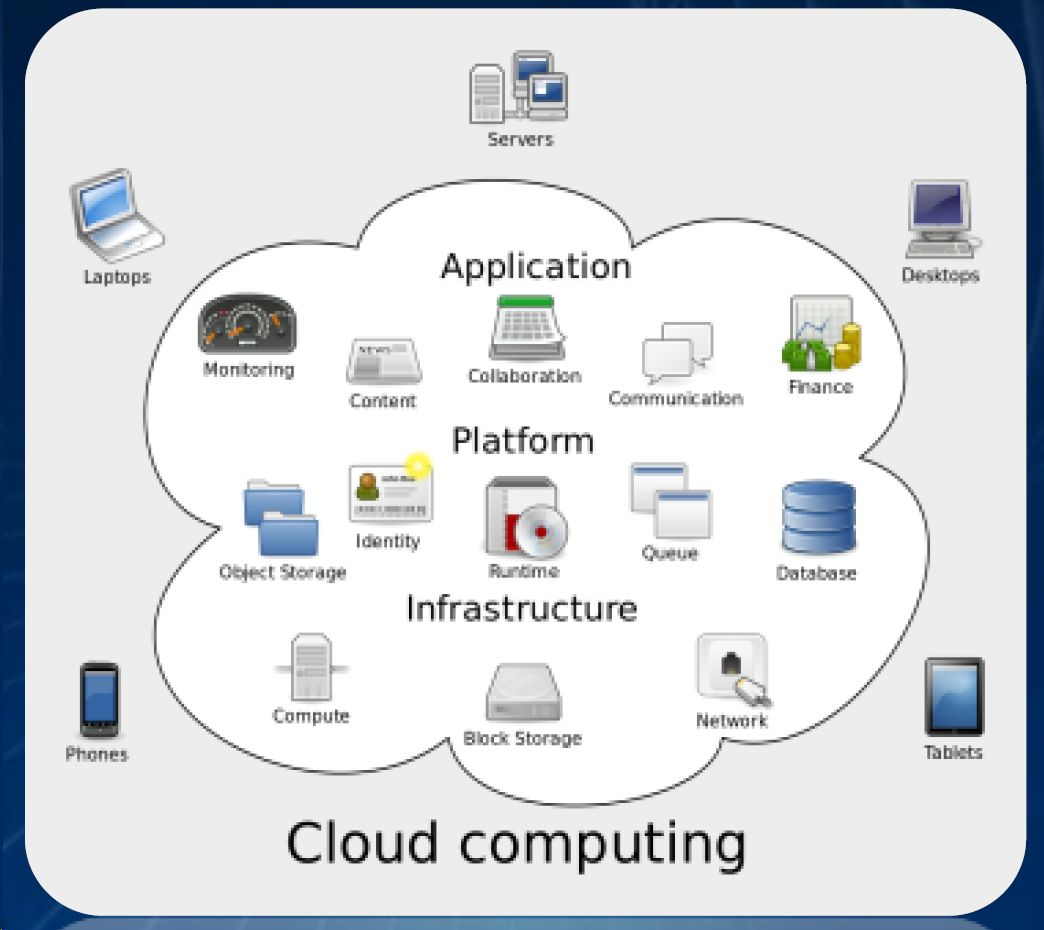
\includegraphics[width=0.7\textwidth]{images/17_lez_fig_01.jpg}
    \caption{Schema dei servizi e modelli del cloud computing.}
    \label{fig:cloud-computing}
\end{figure}

Ecco, vedete cloud computing o nuvola informatica. Ci sono infrastrutture, piattaforme e applicazioni sulle quali vengono gestite le attività più varie, dalla gestione dell'identità, all'archiviazione di oggetti, alla gestione delle reti, attività di collaborazione e quant'altro. 
Alla nuvola accedono i dispositivi più diversi, i server, laptops, telefoni smartphone, tablets e desktop. 

Vediamo adesso un video con delle immagini interessanti che nella maniera migliore può farvi comprendere che cos'è il cloud computing. 

\section{Video e traduzione}
\textit{Hi, today we're going to talk about cloud computing and level 3 communications. It used to be that your key business applications were just down the hall, across the campus, or at your company's headquarters. But now, with cloud computing, business applications, storage, computing cycles, networks, and other services are delivered to users virtually, or in the cloud. 
As your business increasingly relies on cloud computing for services and applications, how do you make sure those applications are as secure and perform as well as they did when they were on your dedicated local or wide area network? That's where the network comes in. Let me explain. Let's start with defining the cloud. Basically, the cloud is a way of delivering applications and IT resources. It's made up of a network of connections that provide access to services and a way for providers to deliver services to users. When you hear someone talk about the cloud, most of the time they are referring to IT services delivered via the public internet. However, many kinds of networks can be referred to as the cloud. There are public clouds based on the public internet, private clouds based on private internets, and hybrid clouds that combine the two. 
Because of the number of versions of the cloud, not everyone is happy with the same one. You might be using an application like email that works fine with the varying performance of the public cloud, but certain users like government agencies, financial institutions, and healthcare providers, to name a few, have serious concerns about privacy and security on the public internet. Not only do users have different needs, but the applications delivered over the cloud have different performance needs as well. What if, for example, you want to use the cloud for telemedicine or to store sensitive data? Would you want your doctor to trust your medical care to a best effort network? With compliance and privacy issues, consistent, secure performance is critical. As businesses migrate more and more critical business functions to the cloud, choosing the right cloud becomes essential. The better the cloud delivers your application and resources, the better your experience. 
If you're planning to use the public cloud, you'll want an internet service provider that can provide high performance and reliability. Level 3 has one of the most connected networks in the world. 60\% of all traffic that originates on the level 3 IP network stays on net. It's like your data is being carried in the express lane on the internet superhighway. When the public cloud simply isn't secure enough or performance is critical, financial institutions, government agencies, and other businesses might be more comfortable with a private cloud. 
This is where level 3 can help. We offer an extensive private IP network, along with other dedicated network options. This allows us to build private or hybrid clouds that offer all the benefits of IP, but with the security and performance of a private network. Cloud computing offers many benefits, but one size cloud does not fit all users. You need the right type of cloud network to support the way you want to use the cloud. 
At level 3, our network is built to offer scalability, performance, and security. 
We provide the platform for businesses to migrate critical applications to the cloud, no matter what type of cloud you require. For more information on cloud computing and how level 3 can help, check out www.level3.com forward slash cloud.}
\\
\\
Ciao, oggi parleremo del cloud computing e delle comunicazioni di Level 3. Un tempo, le applicazioni aziendali fondamentali si trovavano proprio dietro l’angolo, dall’altra parte del campus o nella sede centrale della tua azienda. Ma oggi, con il cloud computing, applicazioni aziendali, archiviazione, cicli di elaborazione, reti e altri servizi vengono forniti virtualmente agli utenti, ovvero nel cloud.

Man mano che la tua azienda si affida sempre più al cloud per servizi e applicazioni, come puoi assicurarti che tali applicazioni siano sicure e performanti quanto lo erano quando si trovavano sulla tua rete locale o su una rete geografica dedicata? È qui che entra in gioco la rete. Lascia che ti spieghi.

Iniziamo col definire il cloud. Fondamentalmente, il cloud è un modo per fornire applicazioni e risorse IT. È costituito da una rete di connessioni che consente l’accesso ai servizi e permette ai fornitori di consegnarli agli utenti. Quando senti parlare di cloud, nella maggior parte dei casi si fa riferimento a servizi IT forniti tramite internet pubblico. Tuttavia, ci sono vari tipi di reti che possono essere definite "cloud".

Esistono cloud pubblici basati su internet pubblico, cloud privati basati su reti private e cloud ibridi che combinano entrambi. A causa di questa varietà di versioni del cloud, non tutti sono soddisfatti della stessa soluzione. Potresti, ad esempio, usare un’applicazione come l’email che funziona bene anche con le prestazioni variabili del cloud pubblico. Tuttavia, alcuni utenti – come enti governativi, istituzioni finanziarie e operatori sanitari, solo per citarne alcuni – hanno serie preoccupazioni riguardo alla privacy e alla sicurezza su internet pubblico.

Non solo gli utenti hanno esigenze diverse, ma anche le applicazioni offerte tramite il cloud hanno requisiti di prestazione differenti. Cosa succede, ad esempio, se vuoi usare il cloud per la telemedicina o per archiviare dati sensibili? Vorresti davvero che il tuo medico si affidasse a una rete “best effort” per curarti? Con le problematiche di conformità e privacy, prestazioni sicure e costanti sono fondamentali.

Man mano che le aziende trasferiscono sempre più funzioni critiche nel cloud, scegliere il cloud giusto diventa essenziale. Più il cloud è efficiente nel fornire le tue applicazioni e risorse, migliore sarà la tua esperienza.

Se prevedi di usare il cloud pubblico, vorrai un provider di servizi internet in grado di garantire prestazioni elevate e affidabilità. Level 3 possiede una delle reti più interconnesse al mondo. Il 60\% di tutto il traffico che ha origine nella rete IP di Level 3 rimane all’interno della rete stessa. È come se i tuoi dati viaggiassero sulla corsia preferenziale dell’autostrada di internet.

Quando il cloud pubblico non è abbastanza sicuro o quando le prestazioni sono fondamentali, istituti finanziari, enti governativi e altre aziende potrebbero preferire un cloud privato. Ed è qui che Level 3 può aiutare. Offriamo un’ampia rete IP privata, insieme ad altre opzioni di rete dedicate. Questo ci consente di costruire cloud privati o ibridi che offrono tutti i vantaggi dell’IP, ma con la sicurezza e le prestazioni di una rete privata.

Il cloud computing offre molti vantaggi, ma una sola tipologia di cloud non è adatta a tutti gli utenti. Serve il tipo giusto di rete cloud per supportare il modo in cui intendi utilizzare il cloud. La nostra rete, in Level 3, è costruita per offrire scalabilità, prestazioni e sicurezza. Forniamo la piattaforma necessaria per consentire alle aziende di migrare applicazioni critiche nel cloud, indipendentemente dal tipo di cloud richiesto.

Per ulteriori informazioni sul cloud computing e su come Level 3 può aiutarti, visita www.level3.com/cloud.




Dal video emerge che il cloud è estremamente complesso e estremamente utile. 
\subsection{Caratteristiche da cui partire}
Quali sono le caratteristiche fondamentali da cui partire:
\begin{itemize}
    \item centralizzazione delle infrastrutture, delle piattaforme e dei programmi informatici, questo è il punto di partenza 
    \item redistribuzione agli utenti finali attraverso internet 
\end{itemize}

\subsection{Modelli di cloud computing}
I modelli noti di cloud sono:
\begin{itemize}
    \item il private cloud
    \item il public cloud
    \item il community cloud
\end{itemize}



Si tratta dei modelli attualmente esistenti, sui quali si fa una distinzione in base agli utenti che possono accedere al sistema. 

\subsubsection{Private cloud}
Nel caso del private cloud, l'infrastruttura è dedicata alle esigenze di un'unica organizzazione e può essere gestita in proprio, in house, oppure può essere gestita da un soggetto esterno che fornisce servizi esclusivamente al cliente, al soggetto che gli ha richiesti. Il private cloud permette di consolidare un'infrastruttura e le applicazioni informatiche che sono necessarie per la gestione delle risorse e per l'erogazione dei servizi a vantaggio di un aumento significativo di efficienza e di efficacia. La scelta della tecnologia da adottare è affidata al responsabile informatico delle singole organizzazioni, in base alle esigenze dell'organizzazione, e può essere dedicata all'infrastruttura a soggetti privati o a soggetti pubblici. 
Quindi si parla di private cloud perché è dedicato ad un unico soggetto e non è aperta ad altri.

\subsubsection{Public cloud}
Nel caso invece del public cloud, l'infrastruttura è di proprietà di un fornitore specializzato in questo specifico ambito tecnologico e il fornitore mette a disposizione degli utenti le risorse utilizzabili per la gestione di attività finali. Sostanzialmente si tratta di un'erogazione di servizi via web e la messa a disposizione di un ambiente nel quale possono essere conservati i dati e al quale si può accedere agevolmente attraverso i propri dispositivi. L'esempio tipico di public cloud è legato ad esempio alla fornitura di web server mail, quindi servizi di posta elettronica a cui si accede direttamente attraverso il web. Il public cloud è generalmente diretto a una molteplicità di utenti che non hanno alcun tipo di rapporto fra loro. 

\subsubsection{Community cloud}
Nel caso invece della community cloud, l'infrastruttura è utilizzata da più utenti che hanno fra di loro degli elementi comuni. Può essere ad esempio una specifica comunità che ha le stesse esigenze e che decide di condividere, di centralizzare, la fornitura dei servizi informatici. L'infrastruttura anche in questo caso può essere gestita dalla stessa comunità oppure anche in questo caso da un fornitore esterno che mette a disposizione le proprie attività, le proprie competenze, i propri servizi a favore della comunità. 

\subsubsection{Cloud intermedi}
Esistono anche dei cosiddetti cloud intermedi nei quali si utilizzano alcune delle caratteristiche di uno, alcune delle caratteristiche dell'altro. 

\subsection{Modelli di servizio}

\begin{itemize}
    \item IAAS, Infrastructure as a Service. In questo caso il fornitore mette a disposizione un'infrastruttura in sostituzione o in aggiunta a sistemi che l'utente ha già a disposizione. Le risorse messe a disposizione dell'utente non sono predefinite, ma sono individuate di volta in volta a seconda delle effettive esigenze che si presentano al momento
    \item SAAS, Software as a Service. In questo caso il fornitore eroga direttamente i servizi, spesso in sostituzione di quelli già installati degli utenti sui loro sistemi e fra i software più diffusi vi sono i fogli di calcolo e gli strumenti per l'elaborazione di testi, di applicazioni di protocollo informatico, per rubriche di contatti, calendari condivisi, sistemi di posta elettronica.
    \item PAAS, Platform as a Service. Nel caso della platform as a service il fornitore offre degli strumenti per sviluppare ed ospitare delle applicazioni nuove ed è un tipo di servizio dedicato soprattutto agli sviluppatori di sistemi. Lo sviluppatore accede alla piattaforma e sulla base di quella sviluppa servizi ulteriori che poi fornisce al soggetto finale. 
\end{itemize}   

Ecco una slide \ref{fig:Cloud_services} che vi può chiarire meglio il funzionamento dei modelli di servizio   

\begin{figure}[ht!]
    \centering
    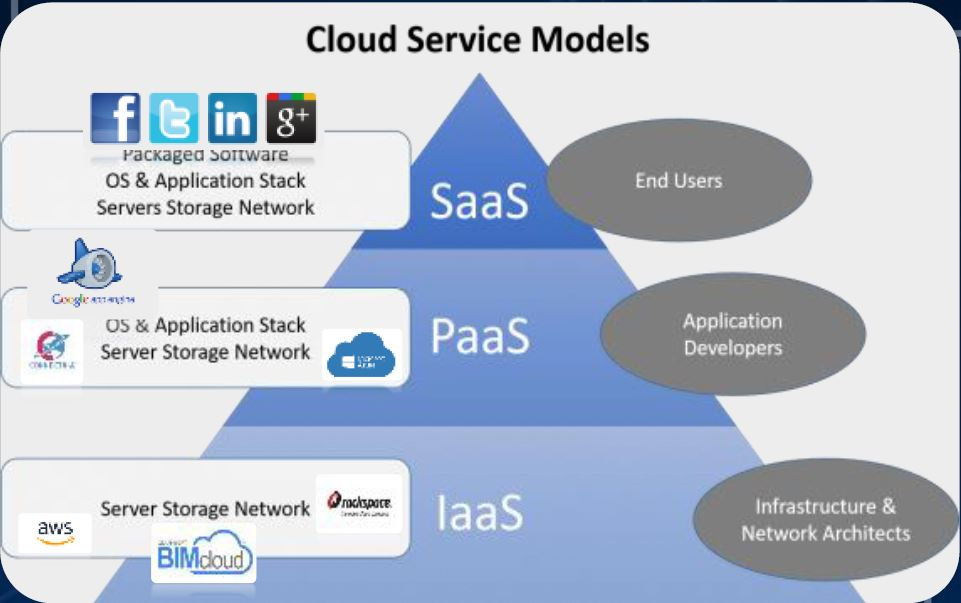
\includegraphics[width=0.7\textwidth]{images/17_lez_fig_02}
    \label{fig:Cloud_services}
    \caption{Cloud services}
\end{figure}

Vedete IAAS, Infrastructure and Network Architettura, trovate qui dei fornitori così per così dire di base, al secondo livello della piramide ci sono gli sviluppatori delle applicazioni, all'ultimo livello della piramide ci sono gli utenti finali che accedono attraverso servizi offerti al pubblico. 

\subsection{Vantaggi del cloud}
Il cloud presenta vantaggi e rischi. 
Vediamo prima di tutto quali sono i vantaggi che sono quelli che hanno portato a una diffusione assolutamente enorme nel mondo odierno dei servizi in cloud: 

\begin{itemize}
    \item acquisire a servizi al posto di acquisire beni con quello che questo comporta dal punto di vista economico
    \item gestione dell'infrastruttura semplificata, effettuata da altri
    \item possibilità di avere un archivio senza limiti di spazio
    \item la possibilità di usufruire di economie di scala
\end{itemize}

Va considerato che la gestione dei sistemi informatici, l'acquisto di sistemi informatici, la loro manutenzione nel corso del tempo, ha dei costi estremamente elevati. 

Una delle caratteristiche della tecnologia moderna è quella di avere un'obsolescenza rapidissima e quindi la necessità di aggiornamento e di adeguamento dei sistemi, sia hardware che software, è una necessità molto forte con richiesta di aggiornamento che è sempre più rapida. Rimanere al passo con i tempi e con gli aggiornamenti richiede degli investimenti economici molto impegnativi. 

La possibilità di accedere a sistemi in cloud consente di ridurre enormemente i costi perché quello che si acquista non è un oggetto, ma sono delle attività, sono dei servizi. 
Quello che si acquista è una licenza di utilizzo, se ci sono degli aggiornamenti che vengono fatti dal fornitore questi aggiornamenti verranno resi disponibili senza necessità di acquisti nuovi ma semplicemente rinnovando e continuando ad avere delle licenze aggiornate. 
Il tema dei costi è un tema fondamentale nella gestione. 

Un altro tema è quello dello spazio, l'archiviazione delle informazioni e dei dati che comunemente si utilizzano nella gestione quotidiana delle attività è enorme. Lo spazio di memorizzazione che si richiedeva un tempo era poca cosa perché si archiviavano soprattutto dati semplici. Oggi con l'utilizzo di programmi complessi e con l'utilizzo di documenti di tipo diverso che prevedono audio, video, prevedono oggetti di grande peso che richiedono un spazio di memoria notevole, anche avere i dispositivi per l'archiviazione ha dei costi e delle richieste di implementazione costante. Anche in questo caso avere a disposizione uno spazio di archiviazione senza la necessità di acquisire la macchina su cui l'archiviazione va effettuata consente di ridurre i costi. 

Altro aspetto riguarda anche la possibilità di fare delle economie di scala. Lo sviluppo di un sistema informatizzato di gestione delle attività personalizzato sul soggetto, sull'organizzazione che ne deve usufruire può avere dei costi anche esso molto elevati. L'utilizzo invece di sistemi sviluppati e resi disponibili a più soggetti consente di facilitare, di dover riflettere meno su quelle che sono le esigenze ma di trovare già un prodotto pronto e anche questo permette delle notevoli economie di scala. Questi sono i vantaggi che hanno portato a uno sviluppo continuo dell'utilizzo dei cloud. 

\begin{figure}[ht!]
    \centering
    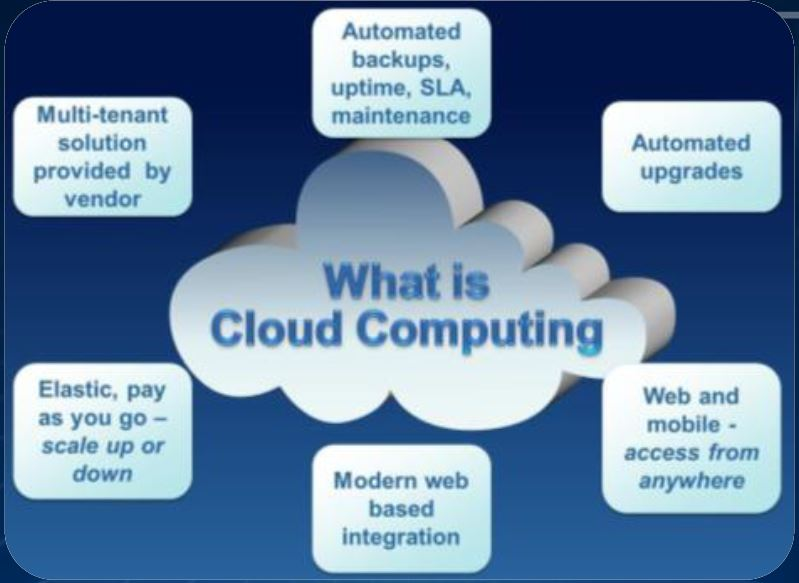
\includegraphics[width=0.7\textwidth]{images/17_lez_fig_03}
    \caption{Vantaggi Cloud}
    \label{fig:Vantaggi_Cloud}
\end{figure}

su questa slide \ref{fig:Vantaggi_Cloud} vedete quali sono le caratteristiche principali e gli aspetti positivi.

\subsection{Rischi del cloud}

Ci sono ovviamente come in tutto ciò che riguarda la tecnologia anche dei rischi. 
Vediamo quindi adesso quali possono essere i rischi dell'utilizzo del cloud:

\begin{itemize}
    \item perdita di controllo sui dati. Il fatto di archiviare i dati su uno spazio che non è proprio ha delle possibilità di rischio rispetto alla loro perdita e questo è un primo tema.
    \item  concentrazione dei dati. Normalmente i soggetti che forniscono servizi in cloud e che quindi archiviano i dati che vengono utilizzati di proprietà dei clienti finali prevedono e provvedono all'archiviazione di dati di più soggetti, di più entità organizzative. Questo significa che in capo ai soggetti, ai fornitori di servizi cloud, si concentrano enormi numeri di dati di più soggetti con il rischio di commistione dei dati se non c'è un sistema di sicurezza adeguato e con il rischio comunque che chi detiene la conservazione dei dati ha un potere immenso perché i dati oggi nella società delle informazioni di oggi sono una ricchezza enorme.
    \item collocazione sconosciuta dei dati. Nel momento in cui noi mettiamo i nostri dati in cloud non sappiamo esattamente dove sono conservati questi dati, dove sono posizionati i server. Nel contratto normalmente è indicato dove sono collocati i server sui quali dati sono archiviati ma la società, il soggetto che fornisce questi servizi nel corso del tempo può subire dei mutamenti e quindi può accadere che questi dati vengano trasferiti altrove. L'utente finale, il cliente che usufruisce dei servizi non sempre può essere messo in condizioni di conoscere dove i propri dati sono archiviati e questo è un tema delicato da trattare. 
    \item  interoperabilità. Il conferimento dei dati su un certo sistema di cloud con determinate modalità può in qualche modo avere dei vincoli. Per avere la disponibilità continua dei propri dati e poter anche decidere di cambiare il fornitore, occorre che i dati vengano conservati in maniera tale che si possano spostare da un punto all'altro. Occorre la possibilità di gestire gli stessi dati anche con un sistema diverso senza avere una perdita. Quindi il tema della interoperabilità è un tema fondamentale nella gestione del cloud.
\end{itemize}

Il primo spunto di riflessione. In cosa consiste il cloud computing? 
%19:40

\section{Cloud computing sostenibile nella strategia europea}

L'importanza che la gestione del cloud ha assunto nel corso degli anni ha portato l'Unione Europea ad occuparsene con diversi programmi di azione. L'Europa ha elaborato delle strategie. 

La strategia generale europea per il cloud computer comporta diversi punti di vista e diverse azioni. 

\begin{figure}[ht!]
    \centering
    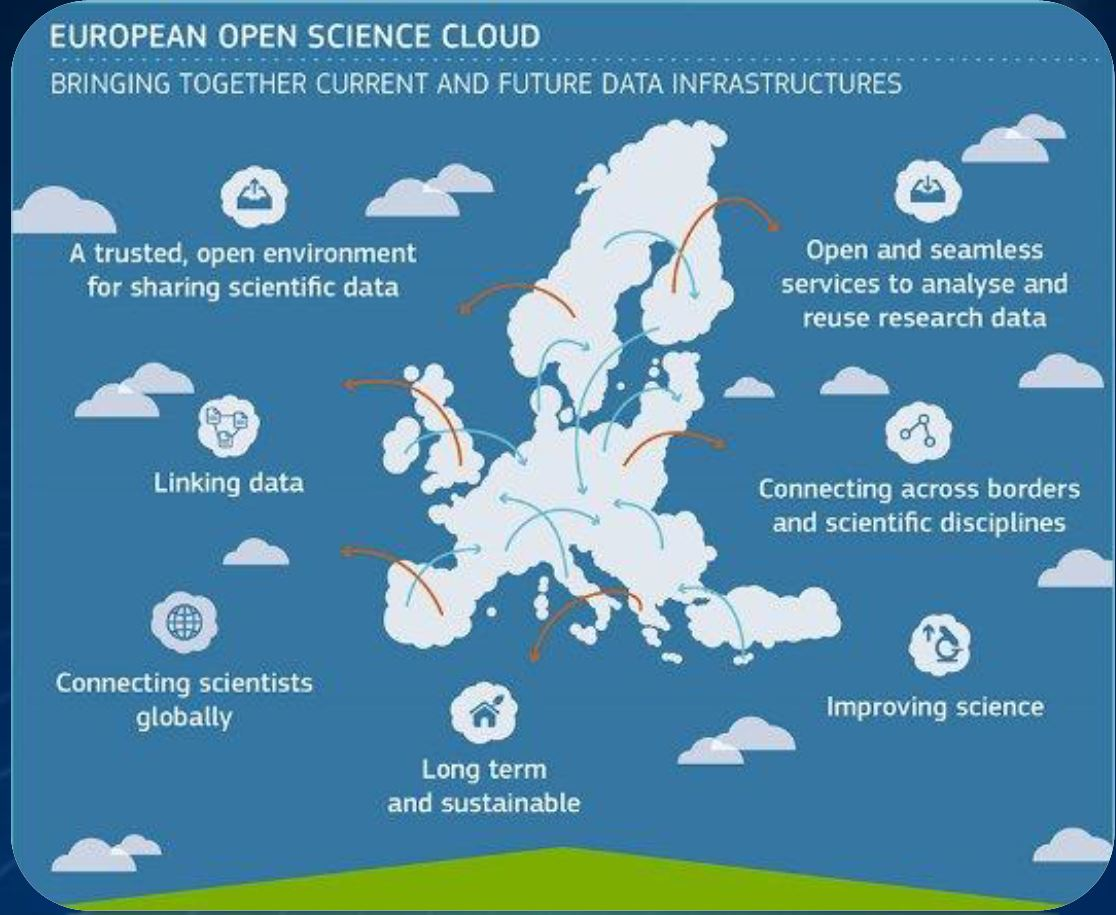
\includegraphics[width=0.7\textwidth]{images/17_lez_fig_04}
    \caption{European open science cloud}
    \label{fig:European}
\end{figure}

Rissumendo possiamo dire che occorre:
\begin{itemize}
    \item un ambiente aperto e affidabile per la condivisione di dati scientifici
    \item un ambiente aperto e gestibile per consentire l'analisi e il riuso dei dati di ricerca
    \item avere delle possibilità di collegamento semplice
    \item andare oltre quelli che sono i confini per poter condividere i dati
    \item una connessione globale tra gli scienziati
    \item una strategia a lungo termine sostenibile
    \item aiutare l'incremento della scienza
\end{itemize}

\subsection{Mercato unico digitale europeo}
La strategia europea attuale passa per un concetto di mercato unico digitale europeo. In questo contesto di mercato unico digitale europeo il cloud computing ha un ruolo chiave per la realizzazione di una data economy europea, di un'economia europea dei dati. 

La realizzazione del mercato unico digitale europeo passa attraverso una regolamentazione ma anche l'adozione, diffusione ed adozione di codici di condotta autoregolatori. 

\subsection{Progetti europei per il cloud}
Un primo progetto europeo, la strategia europea del 2012 per il cloud computing ha fatto partire una serie di iniziative. 

Oggi abbiamo il progetto Horizon 2020 che sta portando avanti i concetti del cloud computing. 

Quindi l'Unione Europea è ormai da diversi anni che si sta occupando di questo tema e nell'occuparsene ha individuato alcuni punti di riferimento fondamentali attraverso i quali bisogna passare per arrivare a quegli obiettivi che abbiamo visto prima. Di base sostanzialmente il concetto è che deve esserci una possibilità di condivisione semplice dei dati all'interno dell'Unione Europea, in particolare dei dati che sono conoscibili a tutti, deve essere possibile consentire a tutti di usufruire della stessa tipologia di servizi in maniera uniforme all'interno dell'Europa, quindi senza digital divide all'interno dei vari paesi europei. Per far questo è stato necessario e occorre continuare a sviluppare delle politiche comuni individuando dei punti di riferimento comuni a cui si possa accedere per proseguire con lo sviluppo. 

Potrete vedere tra i materiali che vi saranno messi a disposizione che ci sono proprio dei siti dedicati dell'Unione Europea proprio per il tema del mercato digitale sostenibile su cui sarà possibile fare degli approfondimenti. 

Vediamo in sintesi quali sono i temi fondamentali. Un cloud computing sostenibile:

\begin{itemize}
    \item richiede l'adozione di regole sicure, uniformi e semplici. Parlare di regole sicure, uniformi e semplici vuol dire uniformare una regolamentazione che è una regolamentazione sostanzialmente giuridica. Abbiamo accennato prima il fatto e poi, tra poco ne parleremo meglio, alla necessità di stipulare dei contratti per accedere ai servizi di cloud. Vedremo tra poco che l'utilizzo del cloud chiama in considerazione una serie di elementi che sono disciplinati da un punto di vista giuridico. Vedremo che abbiamo un tema di trattamento di dati personali, vedremo che abbiamo un tema di gestione dei rapporti contrattuali, vedremo che abbiamo un tema di sicurezza informatica che passa anche attraverso problematiche normative proprio di cyber crime. Quindi c'è un tema giuridico da tenere in considerazione sul quale occorre un'uniformità regolatoria. 
    \item richiede la semplificazione degli standard tecnici. Gestione del cloud è tecnologia e quindi per ottenere una facile circolazione, una facile interoperabilità, occorre avere degli standard tecnici semplificati e condivisibili, quindi due aspetti giuridico e tecnico che non possono in nessun caso essere divisi. 
    \item portabilità dei dati e delle informazioni. Ricordiamoci che i dati, una volta che sono stati strutturati, perché sono stati inseriti all'interno di un sistema, diventano meno flessibili. Per recuperarli e passare ad un sistema diverso, occorre che ci sia la possibilità di uscire, per così dire, da quella che è la struttura nella quale sono inseriti.
    \item interoperabilità
    \item reversibilità, possibilità di tornare indietro nelle informazioni che vengono inserite
\end{itemize}

Quindi l'elaborazione di standard tecnici richiede di tenere in considerazione queste tre caratteristiche, portabilità, interoperabilità, reversibilità. 

Un altro spunto di riflessione: quali sono le regole per un cloud computing sostenibile? 

\section{L'inquadramento giuridico del cloud computing}
Passiamo ora al terzo argomento, l'inquadramento giuridico. L'inquadramento giuridico del cloud computing è determinante per un cloud sostenibile. Per quanto riguarda il fornitore dei servizi di cloud, il fornitore deve:

\begin{itemize}
    \item fornire servizi e consentire l'accesso alla rete
    \item dotarsi di regole contrattuali, gestibili e utilizzabili
    \item occorre prevedere una ripartizione di ruoli e responsabilità nella gestione
\end{itemize}


La disponibilità dei dati e la loro accessibilità in qualunque momento richiede innanzitutto una certezza del livello della connettività. Occorre essere sicuri che sia sempre possibile accedere a quei dati. Provate ad immaginare per un'azienda che decide di usufruire di un servizio in cloud e che quindi archivia tutti i dati che le servono ordinariamente per la gestione dell'azienda su un server cloud e che quotidianamente accede al cloud per la gestione delle attività ordinarie, provate ad immaginarvi se per mezza giornata non è in grado di accedere alle proprie risorse. Questo può creare dei danni anche economici enormi. Quindi occorre avere una certezza sul livello di connettività e la possibilità di accedere ai servizi. È chiaro che l'accesso ai servizi, l'accesso ai dati archiviati, da un lato richiede un'attività del fornitore del servizio, dall'altro passa attraverso l'infrastruttura, cioè attraverso il soggetto che fornisce il servizio di connettività alla rete che normalmente è diverso dal fornitore del cloud. Qua si pone un tema ulteriore e diverso nel quale interviene un soggetto diverso dal fornitore del cloud. 

C'è un tema fondamentale di parità nella possibilità di accesso alle risorse che è in discussione continua. Proprio tra la fine del 2017 e l'inizio del 2018 negli Stati Uniti si è posto il tema della neutralità della rete. Neutralità della rete di cui uno degli aspetti è proprio quello di poter accedere alle risorse indipendentemente da quanto si paga l'accesso alle risorse. Questo è un tema che è importantissimo e che diventerà sempre più importante. 

Secondo tema, come avete visto, sono le regole contrattuali. Nel momento in cui un cliente finale decide di usufruire di servizi informatici in cloud,  di stabilire un rapporto con un fornitore di servizi, lo fa attraverso la stipula di un contratto. 

Contratto che sarà regolato forse dalla normativa nazionale, nella nazione in cui risiede il cliente finale, ma che potrebbe invece essere regolato da normativa diversa se il fornitore dei servizi cloud risiede in un altro luogo. Vedremo fra poco che il tema della giurisdizione, della normativa applicabile, della giurisdizione competente è un tema da affrontare nella parte più concreta, nella gestione più concreta delle attività. 

Ancora, e qua torno al tema del rapporto fra disponibilità del servizio e infrastruttura che mi consente di accedere al servizio, c'è un tema di ripartizione di ruoli e responsabilità per cui se il cliente finale ha un problema deve sapere con chi prendersela. Anche questo aspetto è un aspetto che può essere definito a livello contrattuale ma che può essere definito invece a livello di regolazione generale, normativa generale. 

Altro tema è la sicurezza. Occorre che vi sia un accesso a dati certi e che questi dati siano sempre integri. Il tema dell'accesso e dell'integrità dei dati tocca da un lato il trattamento dei dati personali, dall'altro un tema di sicurezza rispetto alla tutela dei reati informatici.

In entrambi questi casi abbiamo delle normative specifiche. 

Per quanto riguarda il trattamento dei dati personali richiamo il regolamento generale sul trattamento dei dati personali elaborato dall'Unione Europea ed entrato pienamente in vigore nella primavera del 2018. 

Per quanto riguarda i reati informatici, parlando di normativa di carattere internazionale, mi riferisco come punto di riferimento base alla convenzione sul cybercrime elaborata ed emessa a Budapest nel 2001 e che è stata attuata da quasi tutti gli Stati Europei. 

Altro tema è quello della proprietà dei dati, proprietà intellettuale innanzitutto verso open data. 

Quando parliamo di proprietà dei dati parliamo di diversi aspetti. È proprio oggetto di discussione in Unione Europea nella primavera e estate del 2018 una modifica della normativa sul diritto d'autore che ha delle previsioni particolari e che vuole tenere conto delle caratteristiche delle complessità del web. 

Parleremo di questo tema in una prossima lezione. Qua basti dire che il tema della proprietà intellettuale dei dati è un tema che si pone in modo fondamentale nel momento in cui io organizzazione, io soggetto, io cliente finale, conferisco, inserisco i dati all'interno di un sistema di archiviazione di cloud non per questo cedo la proprietà dei miei dati e questo comporta una valutazione, un'elaborazione di norme contrattuali e norme generali che mi consentano di garantirmi rispetto al furto di questi dati o all'utilizzo di questi dati non adeguato. 

Questo è un tema molto dibattuto in rapporto a quelli che sono i cosiddetti open data, cioè i dati che escono in qualche modo dalla sfera di chi quei dati li ha elaborati e di chi è il proprietario dei dati e che vengono messi a disposizione del pubblico. La gestione degli open data è una gestione particolare e articolata che tiene conto di diverse esigenze. 

Si tende a considerare open data quelli che sono i dati di interesse pubblico, si tende a passare agli open data quando il titolare, il proprietario del dato, ritiene che sia possibile metterli a disposizione della collettività. In entrambi i casi vi sono delle normative specifiche condivise a livello internazionale. 

Collocazione e trasferimento dei dati. Abbiamo accennato prima il fatto che i dati non sappiamo dove esattamente vengono collocati. Si pone quindi un tema di giurisdizione, nel caso di contenziosi, e di competenza. 

Altro tema, ne abbiamo accennato prima, è quello dei big data. La conservazione di una grande quantità di dati presso un unico soggetto può porre delle tematiche di concorrenza, può porre delle tematiche di controllo, può porre una serie di temi da affrontare nel momento in cui sono gestite grandi, grandissime masse di dati. 

Ulteriore tema è quello della conservazione. Conservazione dei dati durante il rapporto contrattuale e dopo la scadenza del contratto. Abbiamo visto che nel momento in cui si accede ad un sistema di cloud, nei momenti in cui si archiviano i dati in un cloud, questi dati vengono appoggiati in un sistema di conservazione che esce al di fuori della sfera di disponibilità del soggetto che è proprietario di quei dati o che comunque legittimamente li detiene. Questi dati vengono affidati ad un soggetto terzo in base ad un rapporto contrattuale che stabilisce la regolamentazione del rapporto nella fornitura del servizio e quindi durante quel rapporto contrattuale occorre assicurarsi che i dati vengano conservati in sicurezza, che vengono conservati in maniera da non essere accessibili a terzi che non sono autorizzati a prenderli e ad accedere. Occorre assicurarsi che quei dati vengano messi a disposizione quando c'è la richiesta di accesso a quei dati. 

Nel momento in cui il rapporto contrattuale si chiude, occorre verificare cosa succederà di quei dati. Tipicamente questi dati dovrebbero essere rimessi a disposizione del cliente finale, il quale potrebbe decidere di avvalersi di un altro fornitore. 

Quindi questa parte di gestione dei dati dopo la scadenza del contratto va verificata e disciplinata. 

Avete visto che la gestione del cloud è una gestione complessa dal punto di vista normativo.

Abbiamo visto tra le complessità del mondo moderno vantaggi e svantaggi nell'utilizzo dei sistemi di cloud computing. Ricordiamoci che questi sistemi sono dei sistemi che ormai sono ovunque, sono diffusissimi. Se vedete tutto ciò che chiunque di voi appoggia, per così dire, su uno smartphone, tutti i servizi a cui eccede attraverso uno smartphone, si può rendere conto di come la vita oggi si basi su servizi di cloud. È un sistema eccellente, ma occorre sapere di quali sono le tematiche, quali sono i rischi a cui si va incontro.

Spunto di riflessione: Cosa deve garantire il fornitore di servizi di cloud per rassicurare e assicurare il cliente? 

Abbiamo visto tutta la complessità della gestione del cloud computing e qui facciamo un riassunto, un riepilogo degli spunti di riflessione: 
In cosa consiste il cloud computing? 
Quali regole sono state individuate per un cloud computing sostenibile? 
Cosa deve garantire il fornitore di servizi di cloud? La nostra lezione termina qui. 